% ============================================================
%  Chapter fragment -- included by main.tex
%  (not a standalone document; compile main.tex to build the PDF)
% ============================================================
\begin{multicols*}{3}
\raggedcolumns

\sheettitle{08 -- Malware 1: Types, Rootkits \& Communication}{SWS2 -- ZHAW / Tellenbach}

% ==================== DEFINITION & HISTORY ====================
\section{Definition \& History}
\kw{Malware} = \kw{mal}icious soft\kw{ware}. Comes in many \kw{formats}: executables, shellcode, scripts, firmware.
\begin{itemize}
\item \kw{NIST}: a program \kw{inserted covertly} to compromise \kw{CIA} of the victim's data/apps/OS, or to annoy/disrupt.
\item \kw{Or-Meir et al.}: code whose \kw{presence/behavior the admins are unaware of}; if they knew, they'd not permit it.
\end{itemize}
\textbf{Two main traits (most defs have $\geq$1):} \kw{maliciousness/harmfulness}; acts \kw{without the user's consent/knowledge}.

\subsection{History}
\begin{itemize}
\item \kw{1949} von Neumann -- design for a \kw{self-reproducing} program (theoretical father).
\item \kw{1982 Elk Cloner} -- first \kw{virus in the wild} (Apple II, boot-sector, poem every 50th boot).
\item \kw{1988 Morris Worm} -- first \kw{Internet worm}; 2000 hosts in $<$15h via sendmail/finger/rsh + weak passwords; \kw{multiple infections} slowed hosts to unusable.
\item \kw{2001 Win32.5-0-1} -- first \kw{social-networking virus} (MSN Messenger).
\end{itemize}

% ==================== CLASSIFICATION ====================
\section{Classification}
Helps: \kw{common language} + \kw{risk scoring}. Three lenses:
\begin{itemize}
\item \kw{By type}: main \kw{features} (e.g. replication method) -- bot, virus, worm.
\item \kw{By behavior}: exhibited behavior (e.g. "information stealer").
\item \kw{By family/lineage}: authorship \& evolution (shared/similar code).
\end{itemize}
\hl{No commonly agreed scheme}; some consensus on type characteristics. Categories are \kw{not mutually exclusive} (one sample can be several at once).

% ==================== TYPES ====================
\section{Malware Types \& Terms \hl{(!)}}

\subsection{Trojan Horse}
Sample that \kw{conceals its true identity}. \term{Ex:} whitepaper hiding a PDF exploit; backdoored 3rd-party library; fake printer driver; music player with embedded backdoor.

\subsection{Backdoor \& RAT}
\begin{itemize}
\item \kw{Backdoor}: interactive \kw{1-to-1} access to a compromised host, usually over a \kw{network connection}. \hl{Not} the entry hole itself -- it's what you \kw{plant} to get \kw{back in on demand}, bypassing normal login.
\item \kw{Remote Access Tool (RAT)}: a backdoor with \kw{high interactivity} \& \kw{expansive} access -- sometimes \kw{more powerful} than the normal end-user interface.
\end{itemize}
\textit{Ex flow:} 1) break in once (phish / exploit weak service) $\to$ 2) install backdoor as \kw{auto-start} program $\to$ 3) it \kw{calls home} (\kw{reverse shell} = connects \kw{out}, beats the firewall) $\to$ 4) attacker gets a shell \kw{whenever}, even after the original hole is patched. \textit{(Bind shell = backdoor \kw{listens} on a port, attacker connects in -- needs inbound, rarer.)} \kw{vs Bot} = 1:many via C2; \kw{RAT} = backdoor with rich GUI features.

\subsection{Downloader vs Dropper}
\begin{itemize}
\item \kw{Downloader}: tool whose job is to \kw{download other tools}. Initial stage (spear-phishing) ships a \kw{lightweight} tool that pulls down \kw{feature-full} malware; host attributes \kw{guide} what to fetch. Breaking up the attack \kw{reduces detectability} + enables \kw{surgical retooling}.

\begin{center}
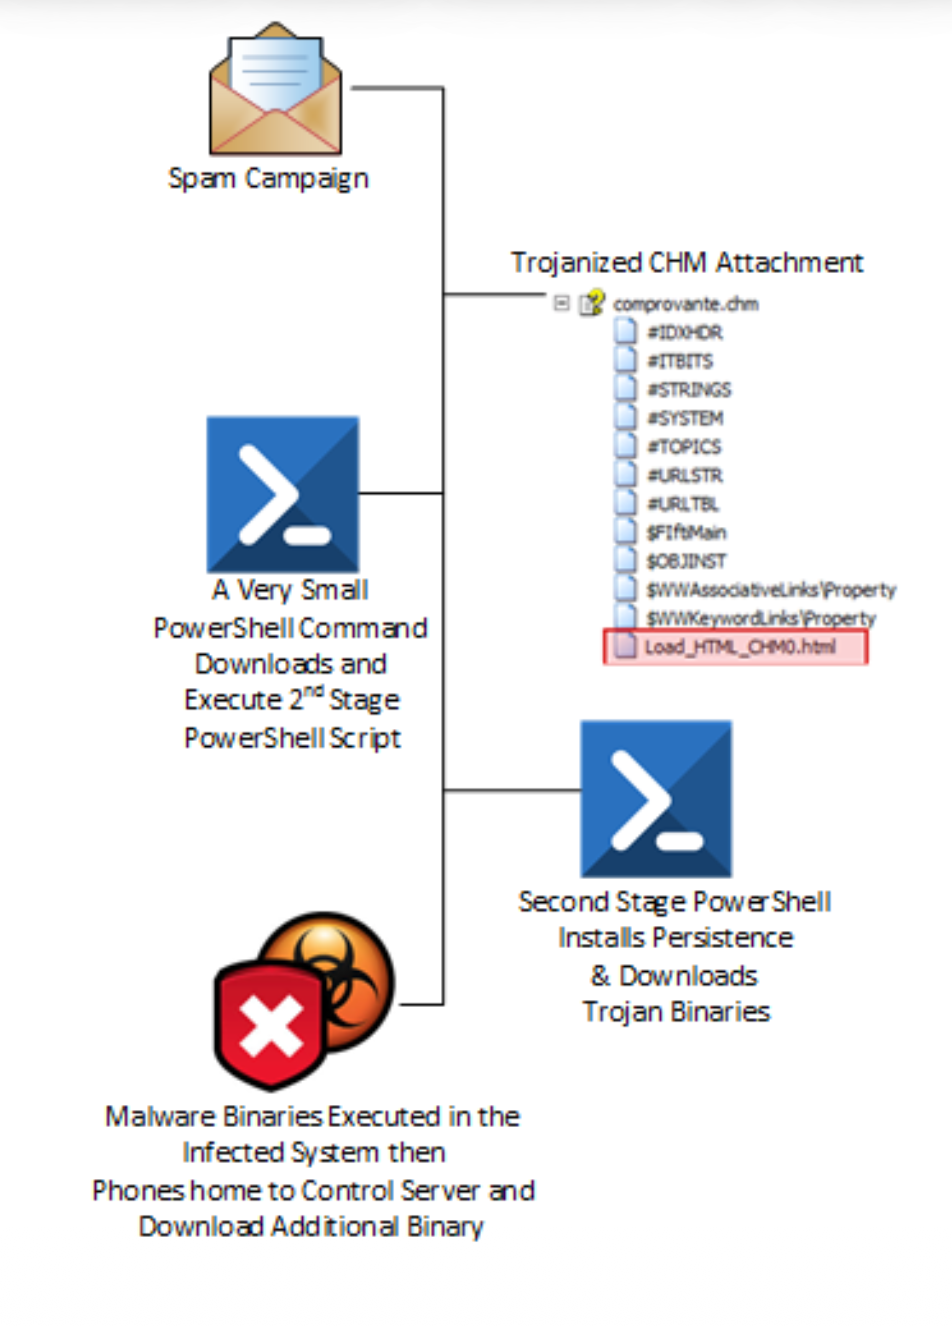
\includegraphics[width=0.4\linewidth]{Figures/downloader_example.png}
\end{center}

\item \kw{Dropper}: \kw{writes/drops} another tool \kw{to disk} \& executes it; the code is \kw{embedded} \& extracted into a native container (e.g. EXE). \term{Ex: HTA with embedded encoded malware.}
\item \hl{Note: downloaders are usually also droppers, but not vice versa.}
\end{itemize}

\begin{center}
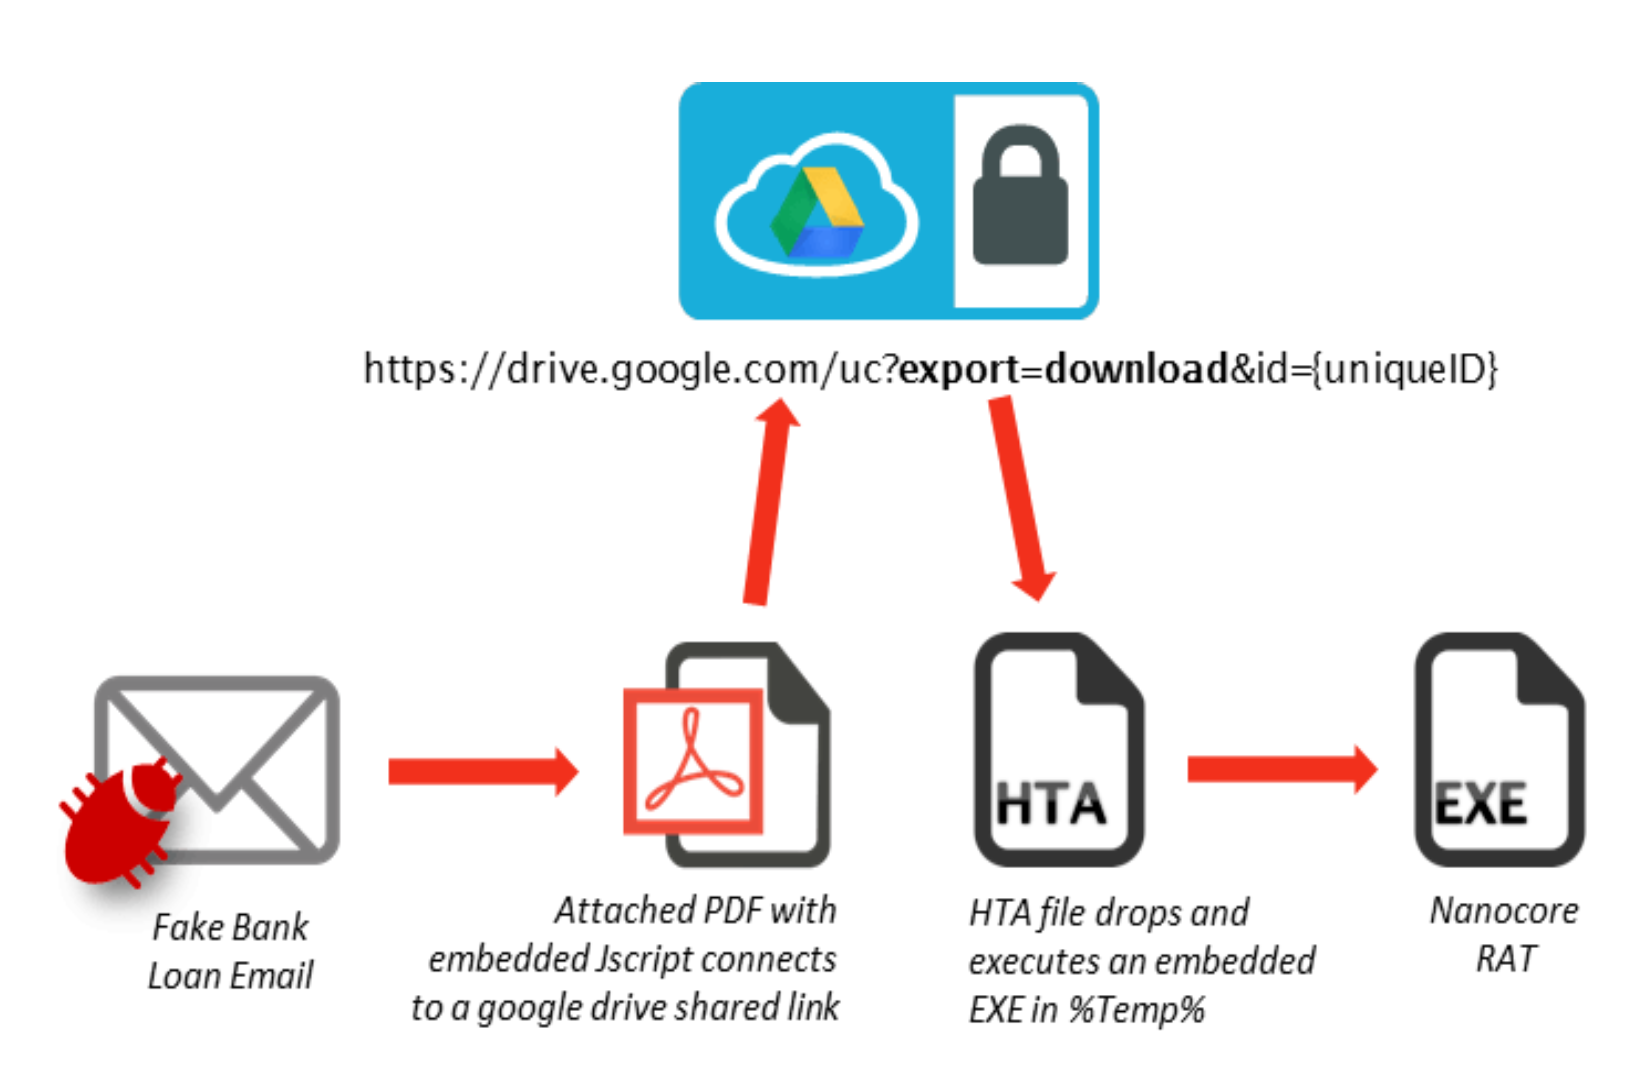
\includegraphics[width=0.4\linewidth]{Figures/dropper_example.png}
\end{center}

\subsection{Bot / Botnet}
\kw{Botnet} = many nodes running a \kw{bot}, coordinated \kw{automatically} or via \kw{C2 (C\&C)} from the \kw{operator}. Like a backdoor but \kw{1:m} (not 1:1) -- one command $\to$ a coordinated army. Uses: \kw{DDoS}, \kw{spam}, credential stealing \kw{at scale}. \term{Ex: Mirai (IoT, default Telnet passwords).}

\textit{Roles (Mirai diagram):} \kw{Bot Master} = operator; \kw{DDoS-for-Hire User} = paying customer; both feed orders to the \kw{C2} (brain, pushes commands down); \kw{Report Server} = nodes report status / new victims; \kw{Malware Loader} = infects newly-found devices; \kw{Botnet Nodes} = the bots sending \kw{attack traffic}.

\textit{Ex flow (self-propagation + attack):} 1) a node \kw{scans} the Internet for devices with open Telnet + \kw{default creds} $\to$ 2) finds one, reports it $\to$ 3) \kw{loader} installs the bot $\to$ new node $\to$ 4) it \kw{scans too} (botnet \kw{snowballs}) $\to$ 5) customer pays Bot Master "take down site X" $\to$ 6) C2 \kw{fans out} the order $\to$ all nodes \kw{flood the victim} = \kw{DDoS}.


\begin{center}
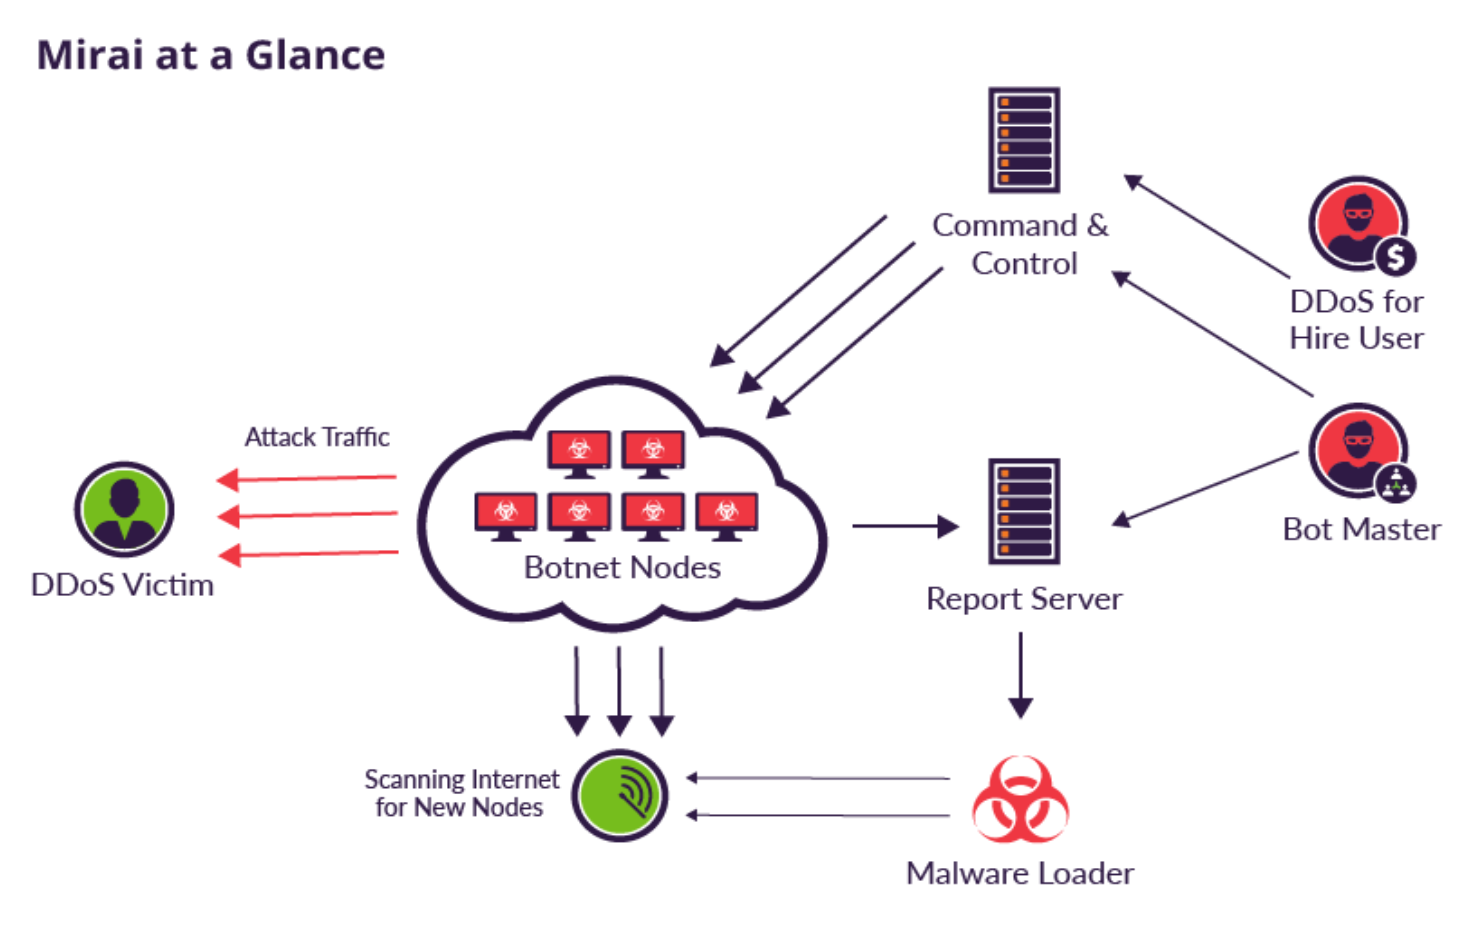
\includegraphics[width=0.5\linewidth]{Figures/mirai_example.png}
\end{center}


\subsection{Spyware -- Monitor vs Info-Stealer}
\begin{itemize}
\item \kw{Monitor}: records user activity/environment $\to$ sends back. Sources: webcam/mic, desktop recording, password prompts, common folders, \kw{keylogging}, browser \& network traffic.
\item \kw{Information Stealer}: \kw{automates} stealing via a \kw{collection plan} (hard-coded / network-provided): contact lists, browser cookies/history, target docs, \kw{credential/keystores}. Like Monitor but with \kw{automated search \& extraction of relevant data only}.
\end{itemize}

\subsection{Scareware / Adware}
\kw{Social-engineering} outcome -- \kw{entice/scare} the user into action. \term{Ex: Fake Anti-Virus} ("you have a virus" $\to$ fake AV $\to$ pay to remove). \kw{Adware} = annoying (popups), \kw{maybe not illegal}.

\subsection{Ransomware}
Like scareware (social-engineer into \kw{paying}), but \kw{encrypts files} then demands money. Modern: strong \kw{public-key crypto} -- malware carries \kw{only the public key} $\Rightarrow$ \hl{practically impossible to recover without paying}. \term{Ex: WannaCry.}

\subsection{Virus vs Worm \hl{(!)}}
Both describe \kw{self-propagating/replicating} malware.

{\footnotesize
\setlength{\tabcolsep}{3pt}
\renewcommand{\arraystretch}{1.15}
\arrayrulecolor{zhawblue}
\noindent\begin{tabular}{@{}>{\raggedright\arraybackslash}p{0.215\linewidth}>{\raggedright\arraybackslash}p{0.35\linewidth}>{\raggedright\arraybackslash}p{0.35\linewidth}@{}}
\rowcolor{zhawblue}
{\color{white}\bfseries} & {\color{white}\bfseries Virus} & {\color{white}\bfseries Worm}\\
\rowcolor{tableblue}
What does it do? & inserts code \kw{into a program/file} (macros, scripts) & exploits a \kw{vulnerability} in app/service/OS\\
\rowcolor{white}
How does it spread? & \kw{users transfer} infected files (run there) & over the \kw{network}, by itself\\
\rowcolor{tableblue}
Infects a file? & \hl{Yes} & \hl{No}\\
\rowcolor{white}
Needs humans? & \hl{Yes} & \hl{No}\\
\rowcolor{tableblue}
Example & \term{Sality} & \term{WannaCry}\\
\end{tabular}}

\textit{In practice the line blurs (email worm/virus).}
\textbf{Famous worms:} \kw{Email worms} (\term{ILOVEYOU} -- 10\% of Internet, 50M in 12 days, $>$\$15B); \kw{Internet worms} scan network/Internet for vulnerable hosts (\term{Code Red, Blaster, SQLSlammer, Conficker}; \term{Witty} = \kw{one UDP packet}); fast-spreading = \kw{no user interaction}.

\subsection{Other terms}
\begin{itemize}
\item \kw{Mailer / Spambot}: sends emails (direct SMTP or victim's webmail).
\item \kw{Cryptominer / Cryptojacking}: mines crypto $\to$ steals \kw{your resources}.
\item \kw{Living Off the Land (LotL)}: uses \kw{already-installed} software for its functionality (e.g. PowerShell, legit remote-mgmt).
\item \kw{Fileless}: \kw{no stand-alone file} -- code lives \kw{only in memory}. Either \kw{in-memory} only (exploit a process \& inject from remote, no FS access) or leverage installed SW to load code into memory (\kw{subset of LotL}).
\end{itemize}

% ==================== ROOTKITS ====================
\section{Rootkits \hl{(!)}}
Use \kw{OS interfaces to conceal} malware's presence (= \kw{stealth}). Variants by where they run:
\begin{itemize}
\item \kw{User-mode} \& \kw{kernel-mode} (below).
\item \kw{Bootkit}: infects \kw{boot sector} (real mode, then kernel mode) $\to$ controls boot, can subvert the kernel.
\item \kw{Hypervisor-level}: uses \kw{HW virtualization} (Intel VT / AMD-V), runs in \kw{Ring -1}, hosts the real OS \kw{as a VM} -- \kw{no kernel modification} needed.
\item \kw{Firmware/hardware}: routers, NIC, HDD, BIOS.
\end{itemize}

\subsection{User-mode (IAT hooking)}
\hl{In plain terms:} programs (Task Manager, Explorer, AV) don't see the PC directly -- they \kw{ask Windows} "what files/processes are here?". The rootkit \kw{sits in the middle of those questions and censors the answer} (removes itself) $\to$ nobody sees it.

\textit{Key terms:}
\begin{itemize}
\item \kw{DLL} (Dynamic Link Library): a \kw{shared library} file of reusable functions that programs call at \kw{runtime} (not compiled into each program). \kw{Kernel32.dll} = core Windows DLL.
\item \kw{Function code}: the actual function inside the DLL.
\item \kw{IAT} (Import Address Table): a table \kw{in the program} of \kw{pointers} ("function $\to$ address"), one per imported function.
\item \kw{EAT} (Export Address Table): a table \kw{in the DLL} listing the functions it offers + their real addresses.
\item \kw{LoadLibrary / GetProcAddress}: Windows functions to load a DLL \& look up a function's address \kw{dynamically} at runtime.
\item \kw{Hook}: redirect a call so it goes through attacker code first.
\end{itemize}

Runs in \kw{user space} / ring 3 (best with \kw{admin} rights -- to write into other processes). Hides processes/files/drivers/ports/services via \kw{function hooking}.

\textit{Reading the diagram -- Normal:} (1, load time) loader copies real addresses from the DLL's \kw{EAT} into the program's \kw{IAT}; (2) program code looks up the function in the \kw{IAT}; (3) the pointer leads to the real \kw{function code} in the DLL. (4--5) dynamic path: code uses \kw{LoadLibrary/GetProcAddress} to resolve an address at runtime.
\textit{Hooked (red):} rootkit overwrites the \kw{IAT pointer} $\to$ points at its \kw{interceptor} $\to$ every call detours through the rootkit, which then calls the real function. It also hooks \kw{LoadLibrary/GetProcAddress} so even \kw{dynamically} resolved calls hit the interceptor. The interceptor \kw{calls the real function, then edits the result}.
\textit{Ex (hide a file):} hook \kw{FindNextFile} $\to$ call the real one $\to$ \kw{strip out} the rootkit's files $\to$ Explorer/AV never see them. \textit{vs kernel-mode: easier to install but \kw{easier to detect} (compare IAT pointers to the DLL's real exports).}

\begin{center}
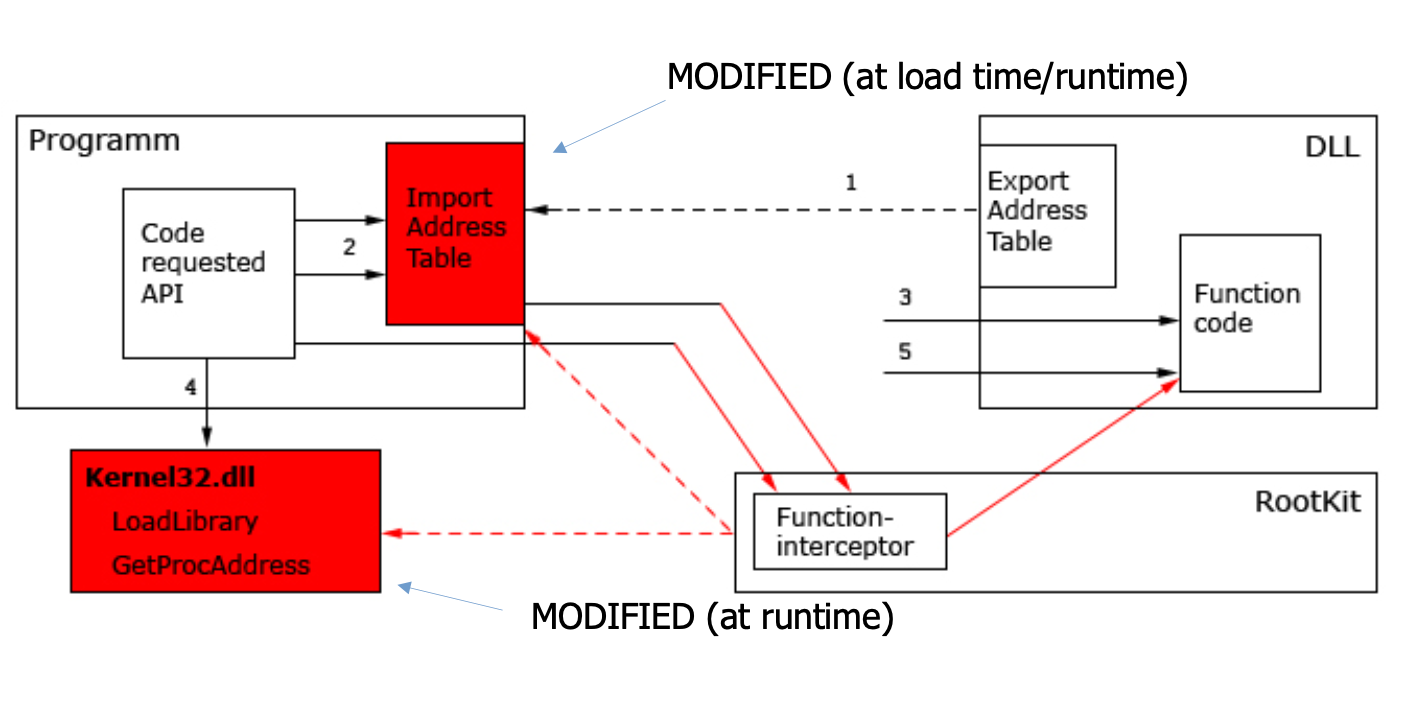
\includegraphics[width=0.8\linewidth]{Figures/user-mode-rootkits.png}
\end{center}

\subsection{Kernel-mode (SSDT hooking)}
\hl{In plain terms:} same "censor the answer" trick, but done \kw{inside Windows itself} (ring 0) instead of in each app -- so it intercepts the questions \kw{deeper down}, where even the IAT-checking AV can't easily see it.

\textit{Key terms:}
\begin{itemize}
\item \kw{Kernel / ring 0}: the core of the OS (full hardware access); apps (ring 3) must ask it via \kw{syscalls}.
\item \kw{Device driver / kernel module}: code that runs \kw{in the kernel}; loading the rootkit = installing a driver.
\item \kw{SSDT} (System Service Descriptor Table): the kernel's \kw{table of pointers} to syscall handlers (e.g. \kw{NtQuerySystemInformation} = "list processes").
\end{itemize}

Loaded as a \kw{device driver / kernel module} $\Rightarrow$ needs \kw{driver-install} rights (admin).

\textit{Reading the diagram -- Normal:} an \kw{SSDT} entry (e.g. \kw{NtQuerySystemInformation}) points straight to the matching function in the \kw{NT OS kernel}.
\textit{Hooked:} rootkit overwrites that \kw{SSDT pointer} to its own \kw{hook} $\to$ the hook calls the real kernel function, then \kw{edits the result} (e.g. removes its process from the list) before returning. Because this is \kw{below} all apps, every program's "list processes/files" call is filtered at the source.
\textit{Deeper = stealthier:} harder to detect than user-mode, but needs to get a \kw{driver loaded} (the main hurdle, see Protections).

\begin{center}
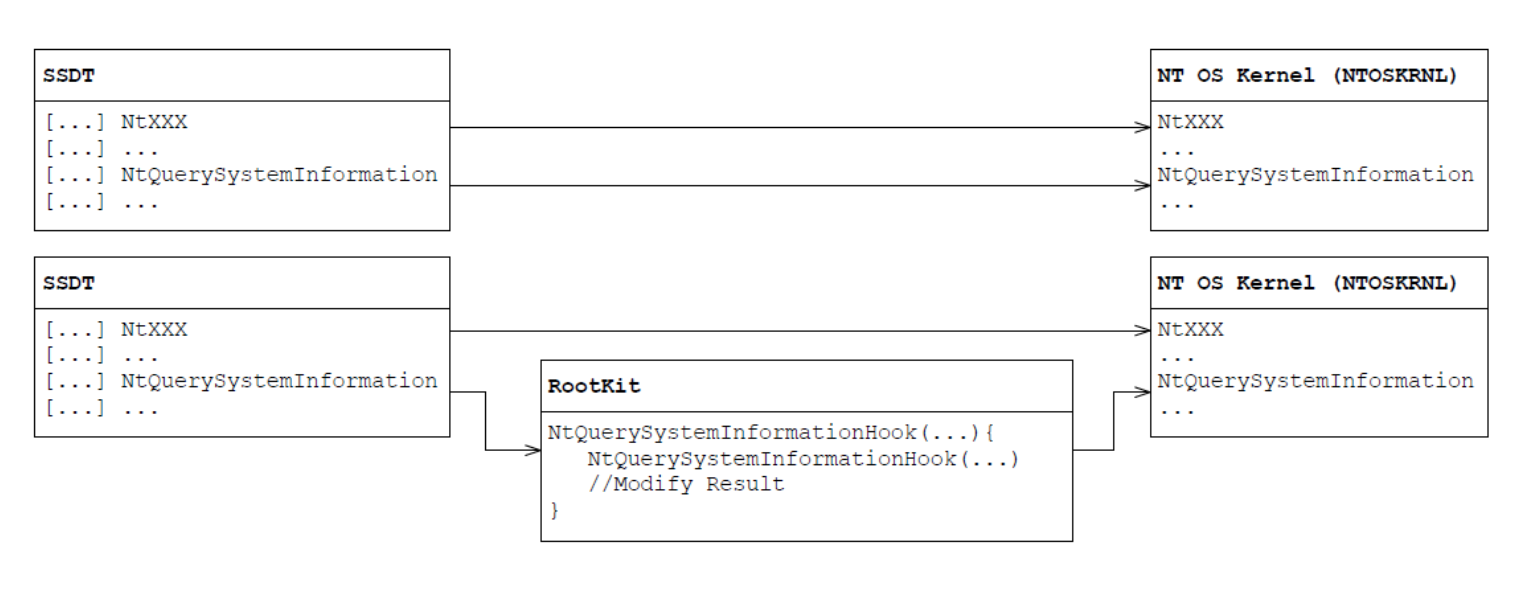
\includegraphics[width=0.9\linewidth]{Figures/kernel-mode-rootkits.png}
\end{center}

\subsection{Protections}
\begin{itemize}
\item \kw{Windows Driver Signing} (Win10+): drivers must be checked \& signed by Microsoft.
\item \kw{PatchGuard} (x64 since XP): prevents modification of structures like the \kw{SSDT}.
\item \kw{Device Guard} (Win10 Enterprise+): only runs code \kw{signed by trusted signers} (per \kw{Code Integrity policy}).
\end{itemize}

\subsection{Detection}
\begin{itemize}
\item Based on the \kw{hiding concept} (e.g. look for \kw{SSDT alteration}).
\item Detecting \kw{sophisticated} rootkits at \kw{ring 0 or lower} is \hl{hard}.
\item \kw{Timing analysis} (generic): hooked/modified ops have \kw{different timing}; \kw{baseline} is the challenge; hypervisor-level needs an \kw{external} time source.
\end{itemize}
\textit{Ex (hypervisor rootkit): \kw{Blue Pill} (Rutkowska 2006) -- AMD-V/Intel VT to move the running OS into a VM \kw{on-the-fly} under a thin hypervisor (VMRUN instruction).}

% ==================== COMMUNICATION ====================
\section{Malware Communication \hl{(!)}}
Many types must talk to the \kw{attacker} or \kw{other instances}. = \kw{communication architecture} + \kw{channel properties}. Goals: \kw{resilient} vs blocking/takedowns; \kw{hard to detect/identify}.

\subsection{Architectures}
\begin{itemize}
\item \kw{Direct}: \kw{attacker} initiates $\to$ malware. \kw{Low} firewall compat (inbound blocked), \kw{easy} takeout.
\item \kw{Client-Server}: \kw{malware} initiates $\to$ \kw{C2} server. \kw{High} firewall compat (outbound allowed), takeout \kw{easy [hard]} (the C2 = single point of failure).
\item \kw{P2P}: either initiates; low-medium firewall compat; takeout \kw{hard} (no central node).
\end{itemize}

\subsection{Killing the C2 (SPOF) \& counter-moves \hl{(!)}}
If the C2's \kw{IP/domain/URL} is known $\to$ \kw{take down / block / sinkhole} it. Malware counters:
\begin{itemize}
\item \kw{Fast Flux}: rotate \kw{IPs} fast (resist IP blocking).
\item \kw{DGA}: rotate \kw{domains} (resist domain blocklists).
\item \kw{Domain Fronting}: hide behind a \kw{clean} domain.
\item Use legit channels (\kw{Dropbox/Evernote}); IRC multiplexing.
\end{itemize}
\textit{Counter-counter: partner with the \kw{registrars} where the criminals bought the C2 domains.}

\subsection{Fast Flux}
\kw{One FQDN} whose \kw{IPs are swapped} in/out rapidly (\kw{TTL $<$300s}) via changing DNS records $\to$ hides a machine behind an \kw{ever-changing set of compromised proxies}; resists IP blocking (\term{Storm Worm 2007}). Defend: block/take down the \kw{FQDN} via registrar.

\subsection{DGA (Domain Generation Algorithm)}
Defeats \kw{bad-domain lists}: algorithm \kw{periodically generates many domains} as \kw{rendezvous points} with the C2. The \kw{huge number} of candidates makes botnet shutdown hard (\term{Emotet}). \textit{Defender can reverse the algorithm to pre-register/block future domains.}

\subsection{Domain Fronting}
Communicate with the C2 using a \kw{totally legitimate domain}: the \kw{TLS SNI} (visible to the firewall) = \kw{benign} domain, but the inner \kw{HTTP Host header} (encrypted) = \kw{malicious} domain. The shared CDN / \kw{DF provider} reads the Host header \& forwards to the real C2 $\to$ firewall only ever sees the benign name.

\begin{center}
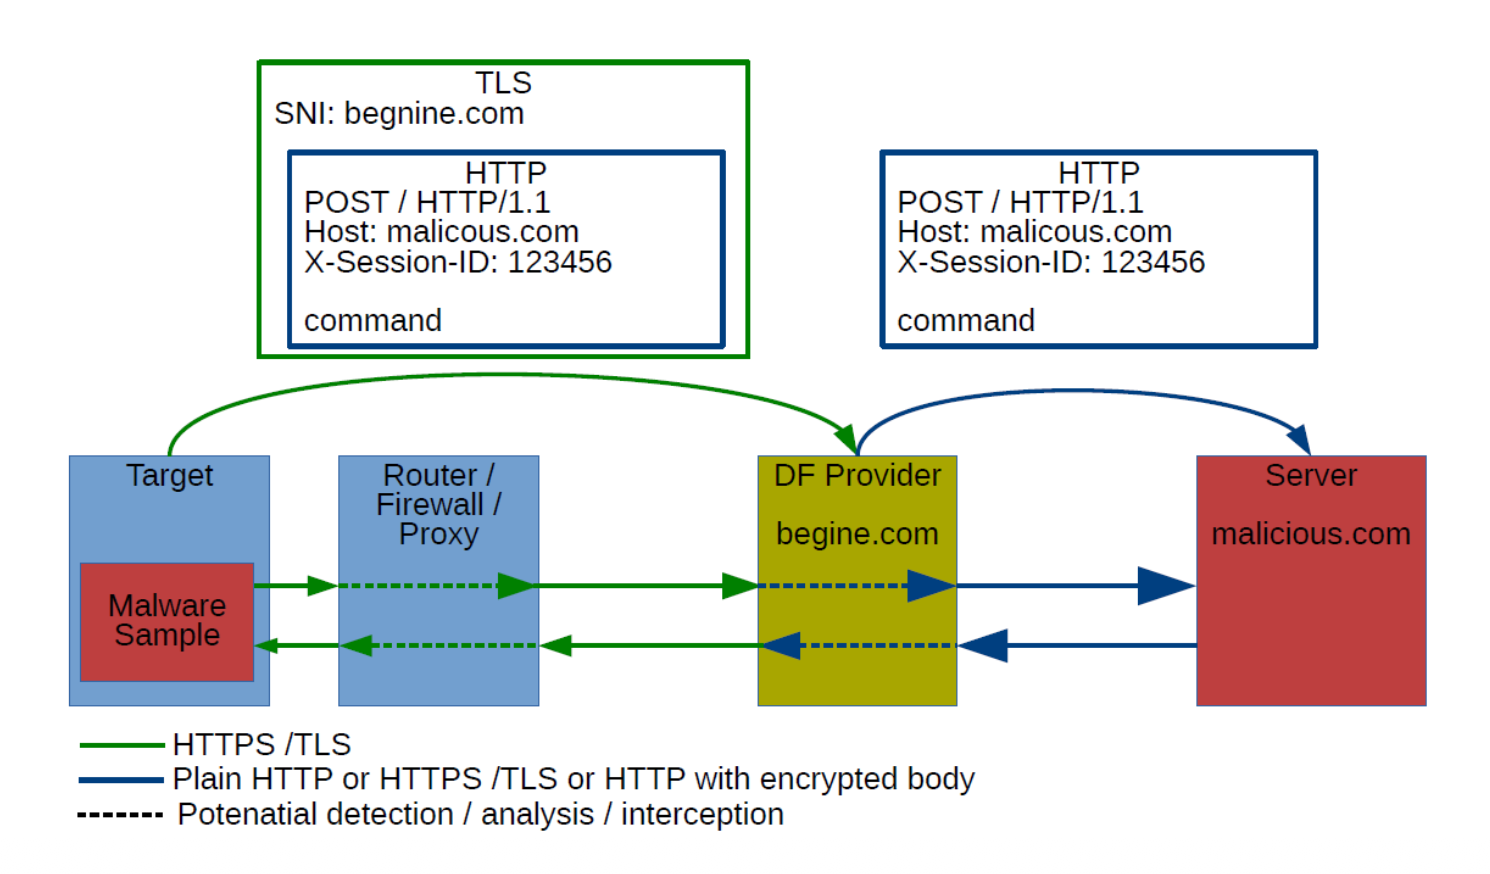
\includegraphics[width=0.8\linewidth]{Figures/domain_fronting.png}
\end{center}

\subsection{Channels}
\begin{itemize}
\item Most common: \kw{HTTPS} (with/without content-level encryption).
\item \kw{Smart exfiltration}: adapt to what's \kw{"normal"} -- which protocols (HTTP/SSH), apps (Dropbox/Citrix), \kw{how much data \& when}.
\item \kw{Side channels}: leak even over an encrypted-only tunnel, e.g. \kw{packet inter-arrival timing} on WLAN.
\item \kw{DNS covert channel}: encode data \kw{in DNS queries/responses} to an attacker-controlled DNS server $\to$ works even when the host is \kw{isolated/firewalled} (DNS usually still resolves). \term{Ex: query \texttt{cl1020-getcmd-...adversary.com}, response IP encodes the command (IP$\to$ASCII).}
\end{itemize}

\begin{defbox}
\textbf{Take-away:} Malware \kw{types} aren't mutually exclusive (Trojan/RAT/downloader/dropper/bot/spyware/ransomware/virus/worm). \kw{Rootkits} hide via OS/kernel/hypervisor; deeper = harder to detect. Communication wants to be \kw{resilient} (Fast Flux, DGA, P2P) \& \kw{stealthy} (Domain Fronting, DNS covert channels). \hl{Defences are still quite weak.}
\end{defbox}

\end{multicols*}
